\chapter{O dado geográfico e seu armazenamento}

De todos os subsistemas de um SIG, o relacionado aos dados é o pilar fundamental que impulsiona os demais. Os dados são o combustível que alimenta o SIG. Esse subsistema é também o mais inter-relacionado, estando inseparavelmente conectado a todos os outros.

\pagestyle{fancy}

\section{Dados e informação. Tipos de informação.}

Há uma diferença importante entre os conceitos de \textbf{dados} e \textbf{informação}. Um SIG é um Sistema de \emph{Informações} Geográficas, mas trabalha com \emph{dados} geográficos — conceitos distintos.

Dado é simplesmente um \textbf{conjunto de valores ou elementos} usados para representar algo. Por exemplo, o código 502132N é um dado.

Esse dado pode ser interpretado como uma coordenada geográfica (latitude 50\textdegree $21'$ $32''$ Norte) ou como um número de identificação. A informação muda, apesar de o dado ser o mesmo.

Assim, \textbf{informação é o resultado da interpretação de um dado}. O trabalho com dados visa, muitas vezes, extrair o máximo de informação possível.

Diferentes dados podem ter volumes diferentes mas conter a mesma informação. Por exemplo, os textos “502132NORTE” ou “CINQUENTA VINTE E UM TRINTA E DOIS NORTE” têm maior volume, mas expressam a mesma informação que “502132N”.

Na informação geográfica, distinguimos duas componentes: \textbf{espacial} (responde a "onde?") e \textbf{temática} (responde a "o quê?").

A componente espacial é geralmente numérica (coordenadas). Já a componente temática pode ser \textbf{numérica} ou \textbf{alfanumérica} (texto). Variáveis numéricas podem ser classificadas como:

\begin{itemize}
\item \textbf{Nominal}
\item \textbf{Ordinal}
\item \textbf{Intervalar}
\item \textbf{De razão}
\end{itemize}

O tipo de variável determina as operações possíveis em um SIG.

Outro conceito importante é a \textbf{dimensão} dos elementos (ponto = 0D, linha = 1D, polígono = 2D, volume = 3D), como mostrado na Figura~\ref{Fig:Dimensiones}.

\begin{figure}[!hbt] 
\centering
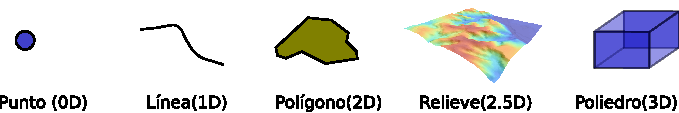
\includegraphics[width=\textwidth]{dados/Dimensiones.pdf}
\caption{\small Dimensões da componente geográfica.}
\label{Fig:Dimensiones} 
\end{figure}

\section{Divisão da informação: Camadas}

Em SIG, a informação espacial de uma região é \textbf{dividida em camadas} temáticas independentes (Figura~\ref{Fig:Concepto_capa}).

\begin{figure}[!hbt] 
\centering
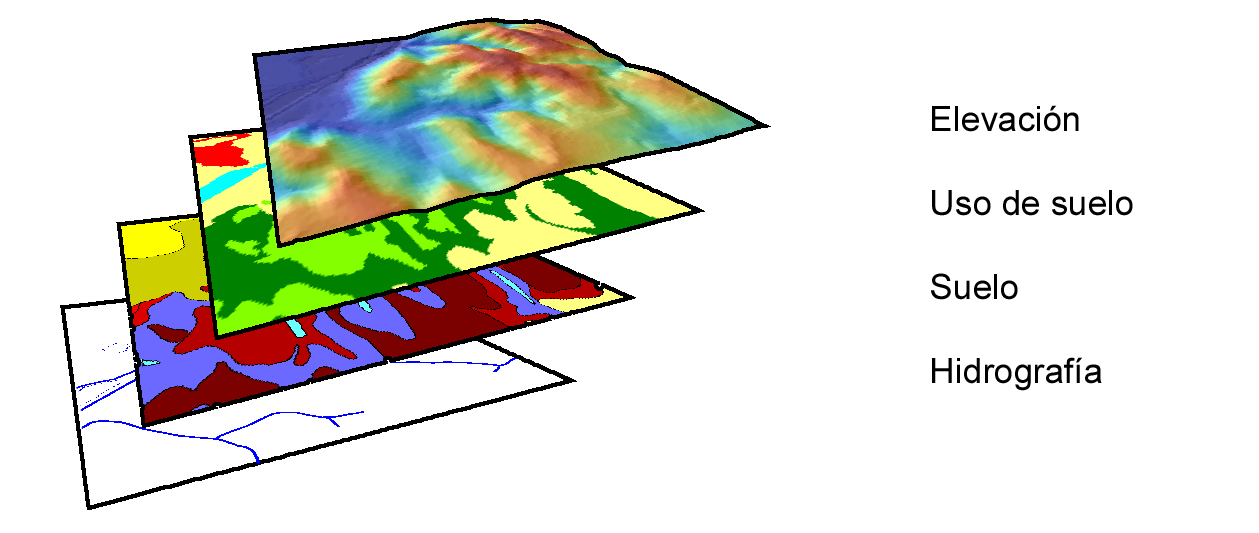
\includegraphics[width=\textwidth]{dados/Concepto_capa.png}
\caption{\small Conceito de \emph{camada} de informação geográfica em um SIG.}
\label{Fig:Concepto_capa} 
\end{figure}

O conceito de camada é essencial. Cada camada pode ser visualizada e manipulada separadamente. Diferentes tipos de informação são combinados facilmente, ao contrário da cartografia impressa.

Camadas também permitem versões de dados para diferentes escalas. Evitam redundância, já que cada camada armazena apenas um tipo de informação.

Além da divisão temática, os dados podem ser subdivididos espacialmente — como folhas de mapas impressos. A separação entre \textbf{dados e visualização} permite montar mosaicos a partir de diferentes fontes.

\section{Modelos de informação geográfica}

Transformar uma área geográfica em dados SIG envolve:

\begin{itemize}
\item \textbf{Modelo geográfico} — representação conceitual da realidade.
\item \textbf{Modelo de representação} — forma de descrever o modelo geográfico.
\item \textbf{Modelo de armazenamento} — estrutura para guardar os dados.
\end{itemize}

Os modelos de representação mais comuns em SIG são:

\begin{itemize}
\item \textbf{Raster}
\item \textbf{Vetorial}
\end{itemize}

\subsection{Modelo raster}

Divide o espaço em uma \textbf{malha regular} de células (Figura~\ref{Fig:Raster_closeup}).

\begin{figure}[!hbt]   
\centering
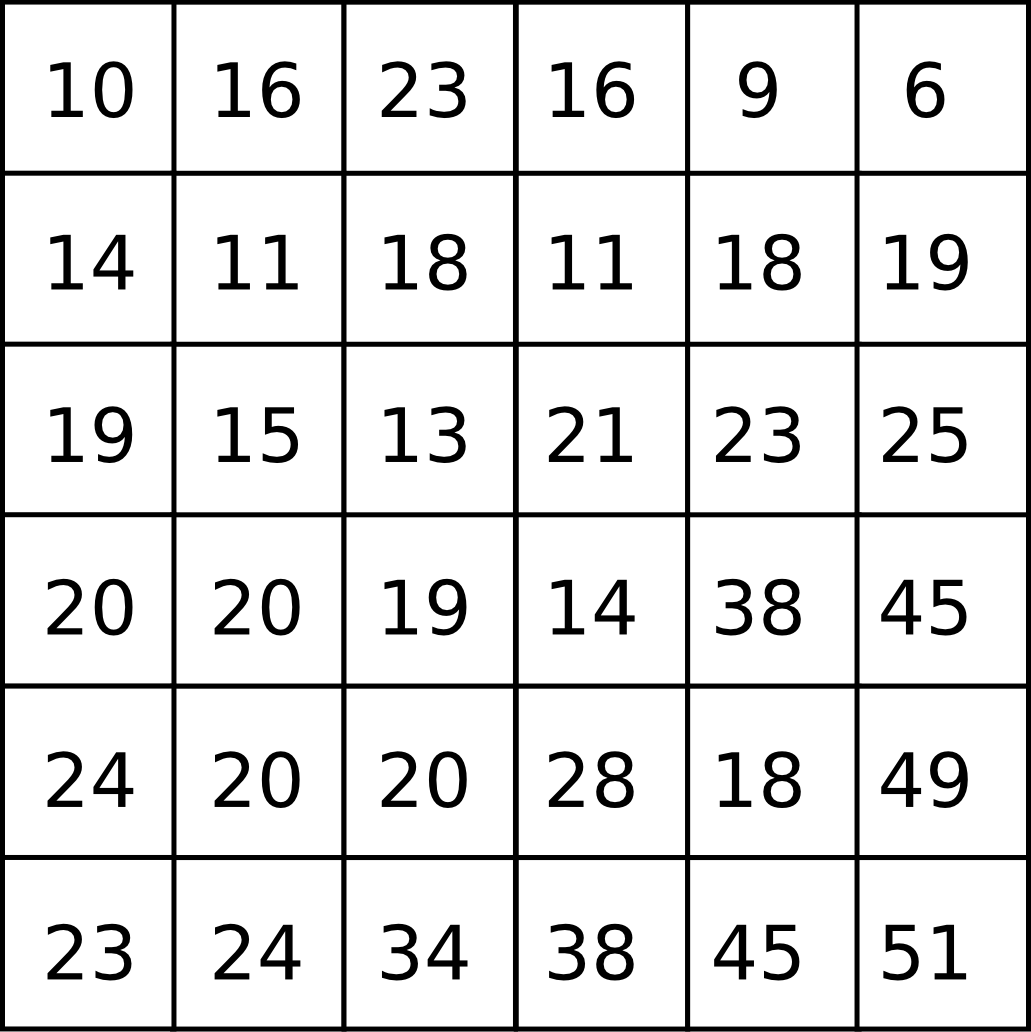
\includegraphics[width=.4\textwidth]{dados/Raster_closeup.png}
\caption{\small Células de uma malha raster com seus valores.}
\label{Fig:Raster_closeup} 
\end{figure}

Cada célula tem um valor numérico, geralmente em uma ou mais \textbf{bandas}. Imagens digitais e Modelos Digitais de Elevação (MDE) são exemplos de uso do modelo raster.

Cada raster pode ser tratado como uma \textbf{matriz}, facilitando análises matemáticas.

\subsection{Modelo vetorial}

Baseia-se em \textbf{entidades geométricas} (ponto, linha, polígono) — ver Figura~\ref{Fig:Primitivas_vectoriales}.

\begin{figure}[!hbt]   
\centering
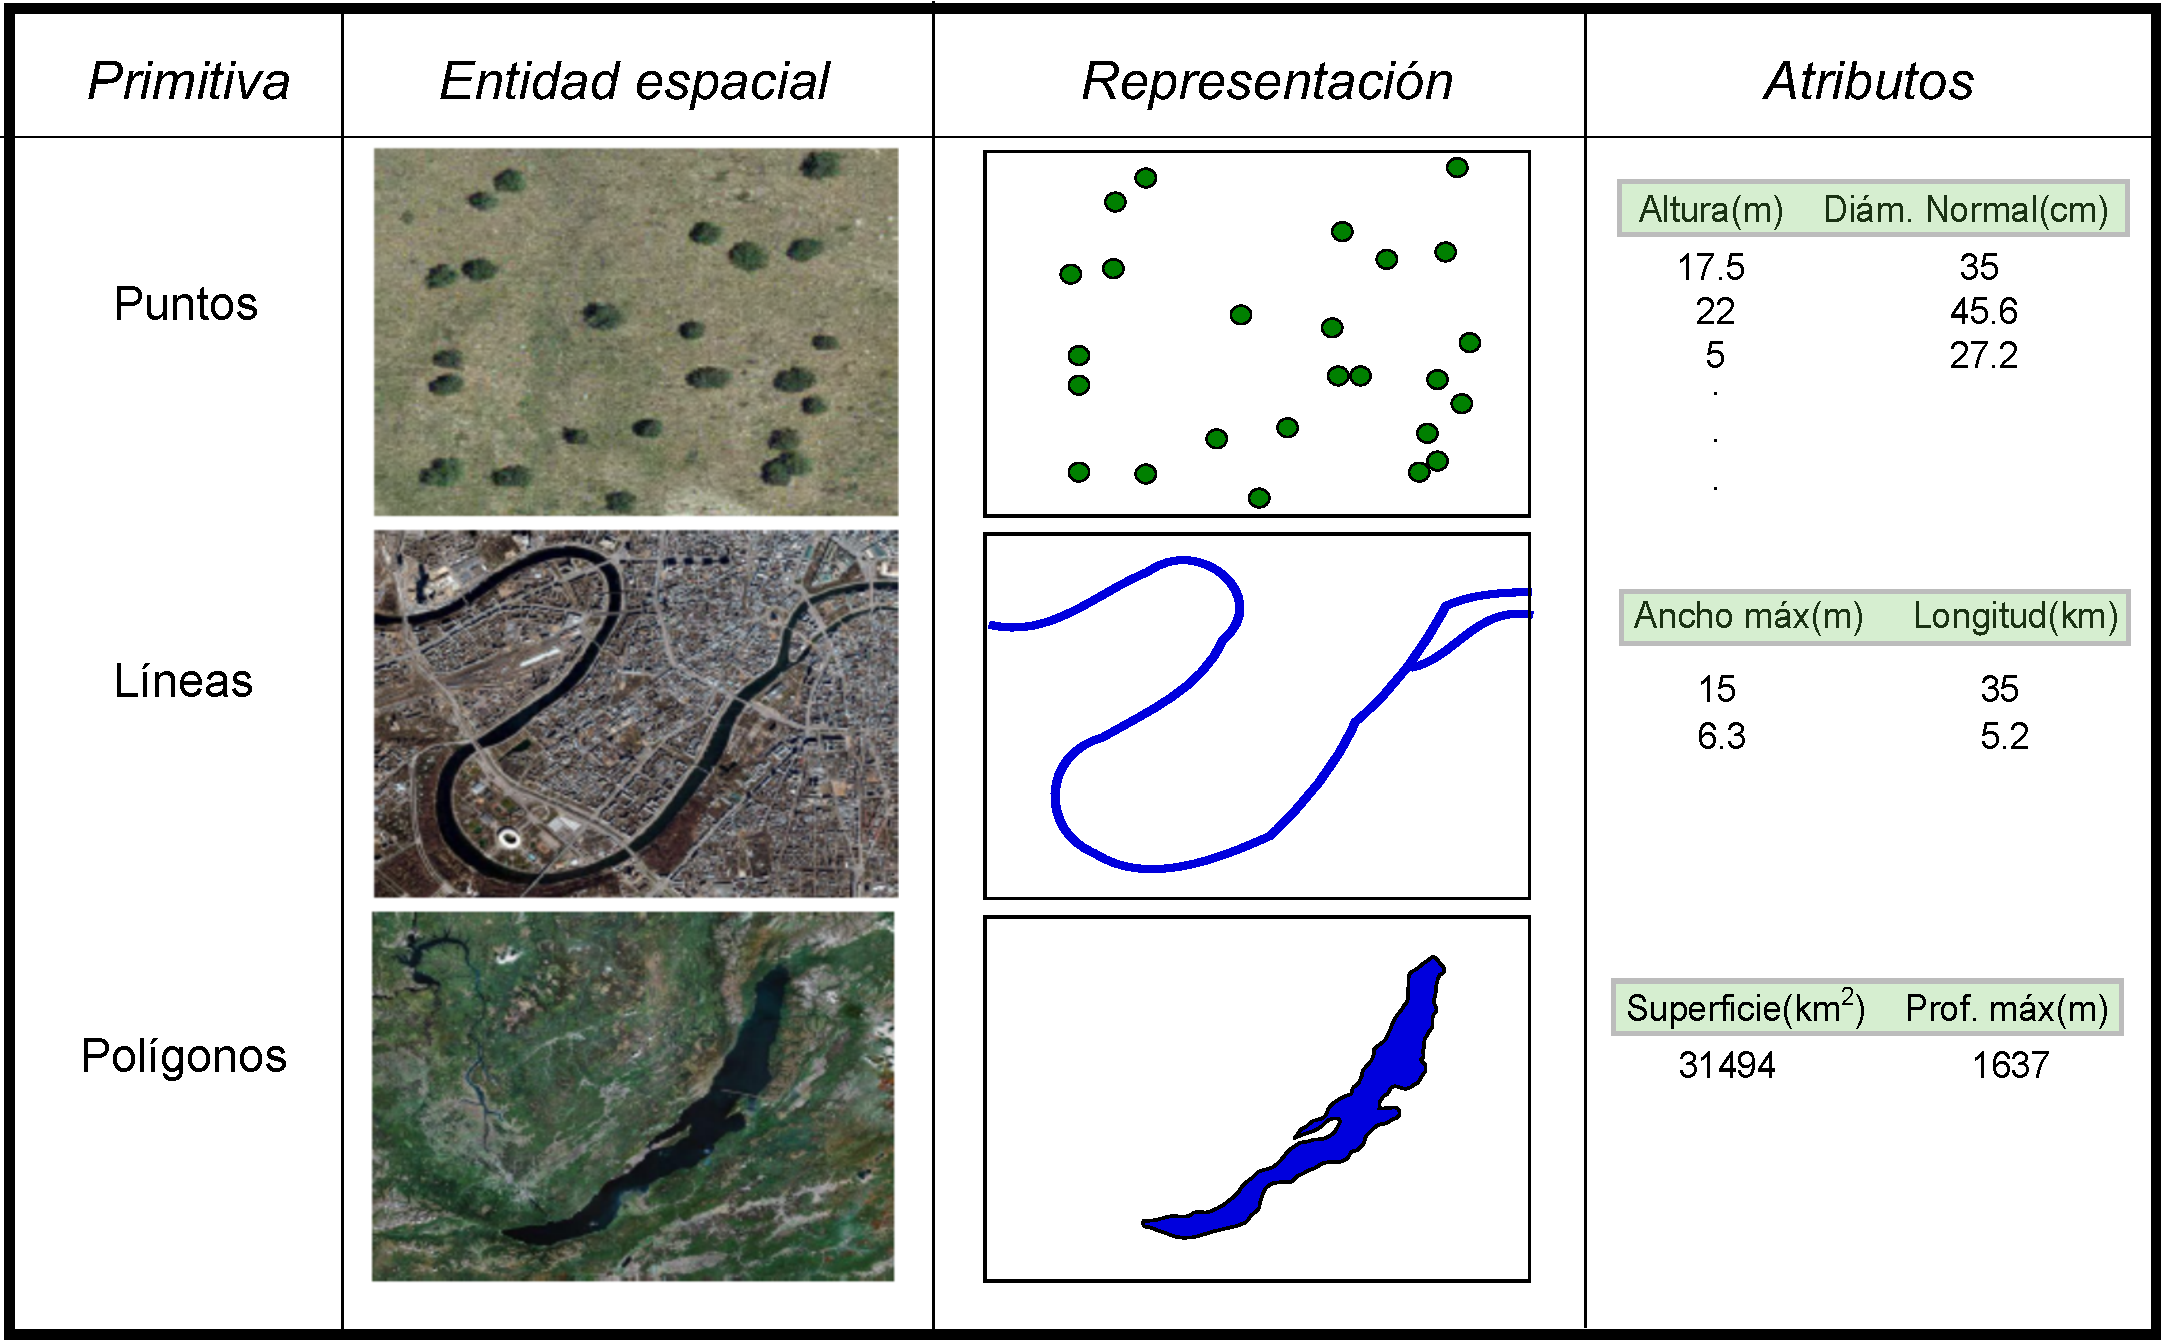
\includegraphics[width=\textwidth]{dados/Primitivas_vectoriales.pdf}
\caption{\small Primitivas geométricas e exemplos de atributos.}
\label{Fig:Primitivas_vectoriales} 
\end{figure}

Cada entidade pode ter múltiplas primitivas e diversos \textbf{atributos}, armazenados em tabelas (bancos de dados). Esses atributos podem ser analisados independentemente da geometria.

A \textbf{topologia} armazena relações espaciais entre entidades, sendo essencial em análises como redes viárias (Figura~\ref{Fig:Topologia_vias}).

\begin{figure}[!hbt]   
\centering
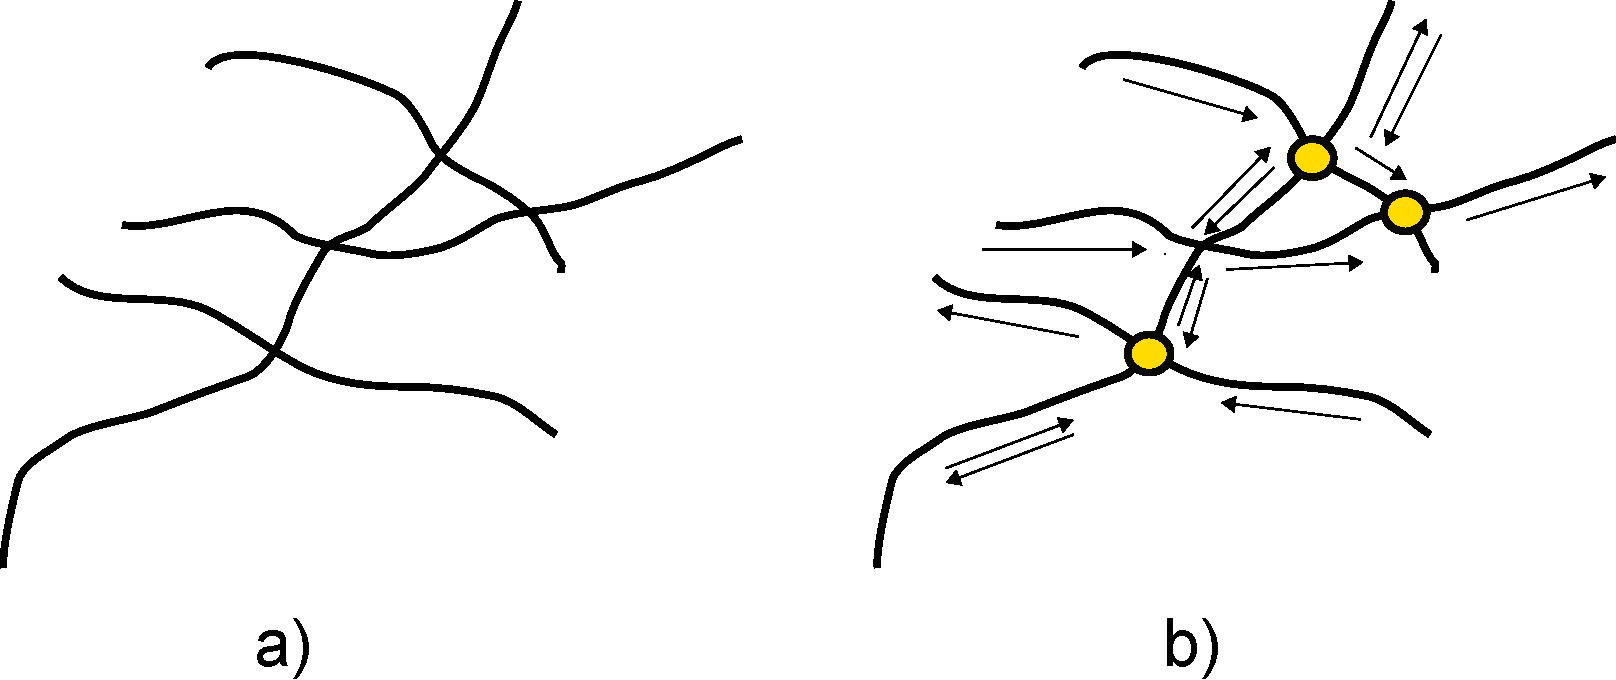
\includegraphics[width=.8\columnwidth]{dados/Topologia_vias.pdf}
\caption{\small Camada de vias sem (a) e com (b) topologia.}
\label{Fig:Topologia_vias} 
\end{figure}

Sem topologia, as entidades vetoriais são tratadas como um \emph{espaguete} — sem relações entre si.

\subsection{Raster \emph{vs} Vetorial}

Ambos os modelos podem representar qualquer tipo de informação (Figura~\ref{Fig:Esquemas_modelos_representacion}).

\begin{figure}[!hbt]   
\centering
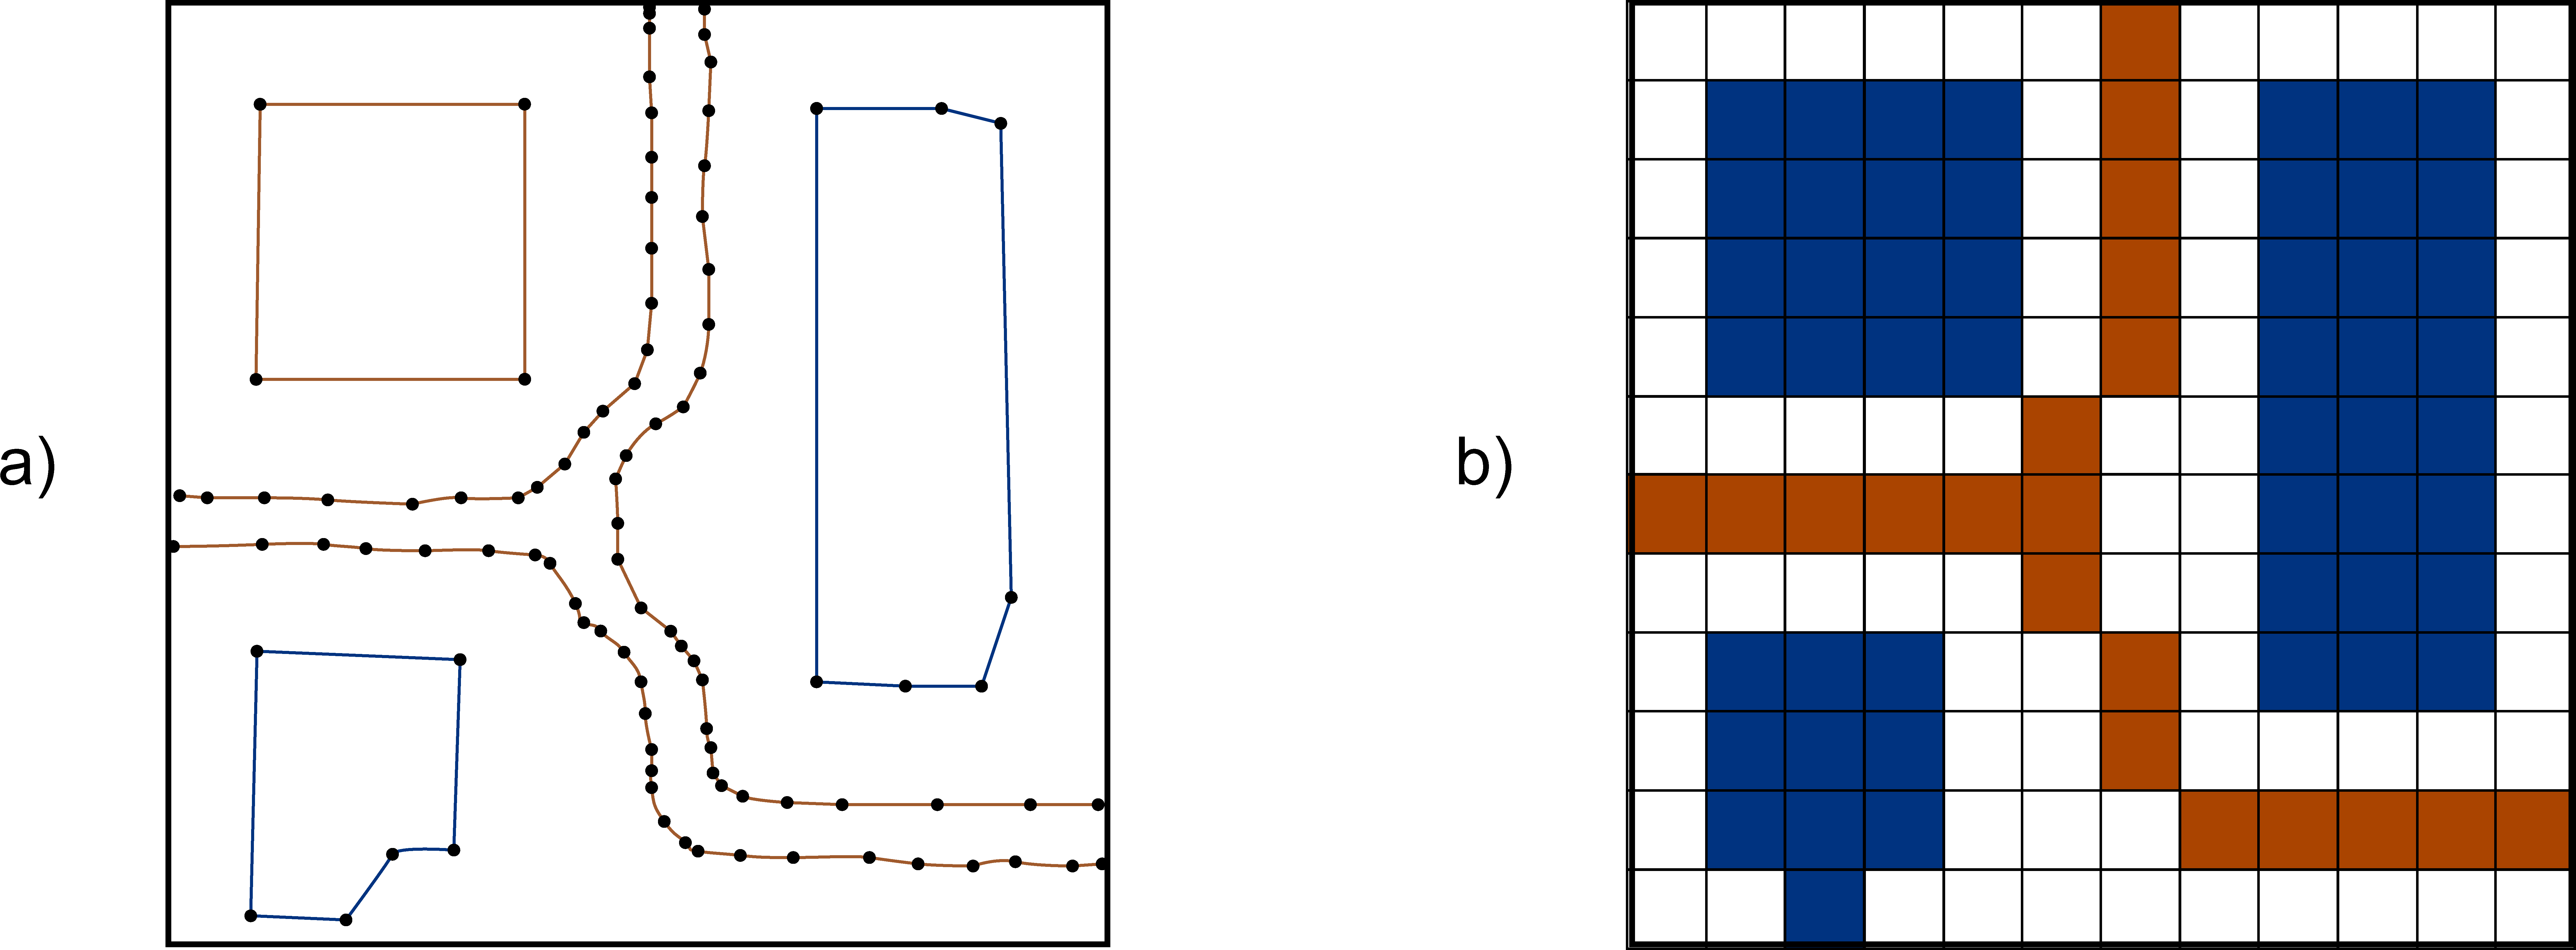
\includegraphics[width=\textwidth]{dados/Esquemas_modelos_representacion.pdf}
\caption{\small Comparação entre representação vetorial (a) e raster (b).}
\label{Fig:Esquemas_modelos_representacion} 
\end{figure}

Comparação:

\begin{itemize}
\item \textbf{Enfoque}: Raster enfatiza o \emph{o quê}, vetorial o \emph{onde}.
\item \textbf{Precisão}: Raster é limitado pelo tamanho da célula (Figura~\ref{Fig:Imprecision_raster}); vetorial tem maior precisão nas formas.

\begin{figure}[!hbt]   
\centering
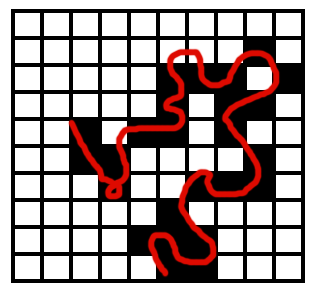
\includegraphics[width=.4\columnwidth]{dados/Imprecision_raster.png}
\caption{\small Limitação de forma no modelo raster.}
\label{Fig:Imprecision_raster} 
\end{figure}

\item \textbf{Complexidade}: Algoritmos de análise são mais fáceis de implementar em raster.
\end{itemize}

Não há modelo ideal absoluto. A escolha depende de:

\begin{itemize}
\item \textbf{Tipo de variável}: contínua (ex: elevação) → raster; discreta → vetorial.
\item \textbf{Tipo de análise}: raster para cálculos, vetorial para visualização.
\item \textbf{Contexto}: imagens sempre em raster.
\end{itemize}

É possível \textbf{converter} entre modelos conforme a necessidade da aplicação.

\pagestyle{empty}
